\chapter[The HADES Oracle database]{The HADES Oracle database} \label{ch:oracle}

\section[Overview]{Overview}

The HADES database is the central place, where information and parameters from the various systems flow together:
the file catalog is filled by the DAQ and the EPICS slow control data are stored online.
\begin{figure}[\htb]
  \centering
  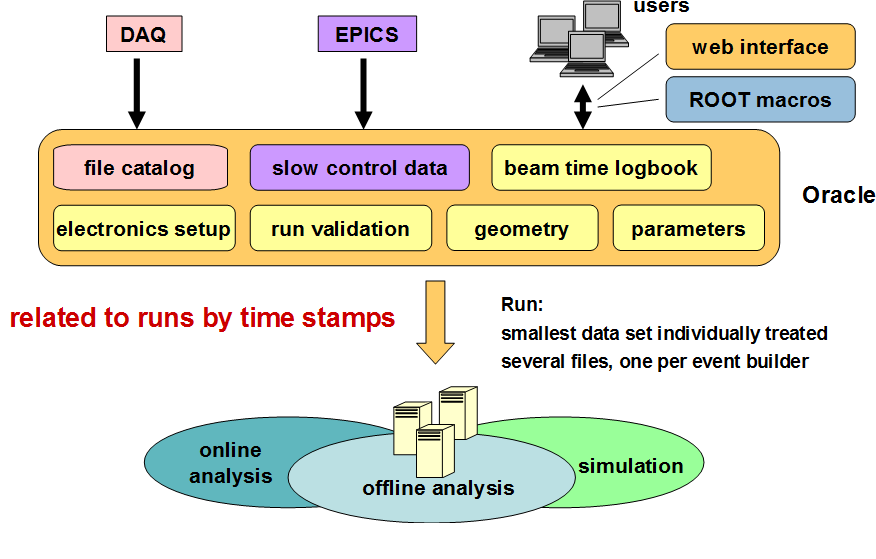
\includegraphics[scale=0.50]{hydra2_ora_overview.png}
  \caption[Overview]{ Overview} \label{fig:oraOverview}
\end{figure}

Many users store and retrieve data either by programs or web interfaces: the beam time logbook, information about the 
detector hardware and electronics setup, the run quality, the geometry and alignment, analysis parameters and conditions.\\
All these data are related by timestamps.


\section[The version management of parameter containers]{The version management of parameter containers} 
\label{sec:oraVersionmanagement}
Most parameters used by the analysis change over time and need a version management in Oracle. Some data can have only one 
valid value at a certain date as for example the position of a certain cable, other ones may even change over time for a 
certain DAQ or simulation run depending on the status of the analysis (different generations of DST productions).\\

The major requirements are:
\begin{itemize}
 \item It must be possible to get a consistent set of parameters at any date.
 \item To keep the history, no information, even if it is wrong, should to be overwritten without trace, to get an answer on 
       questions like this: \textit{``Which parameters have I used when I did the analysis of these runs six months ago?''}
 \item Good performance
\end{itemize}

All tree- and condition-style parameter containers have a \textbf{three dimensional version management} 
(fig:~\ref{fig:oraVersionmanagementParameters}):
\begin{enumerate}
  \item time axis of runs
  \item time axis of history
  \item parameter context
\end{enumerate}
A version is valid for a certain time range on the runs axis and on the history axis (defines a 2-dim plane) and for a 
specific parameter context (different 2-dim planes with individual time ranges).\\

\begin{figure}[\htb]
  \centering
  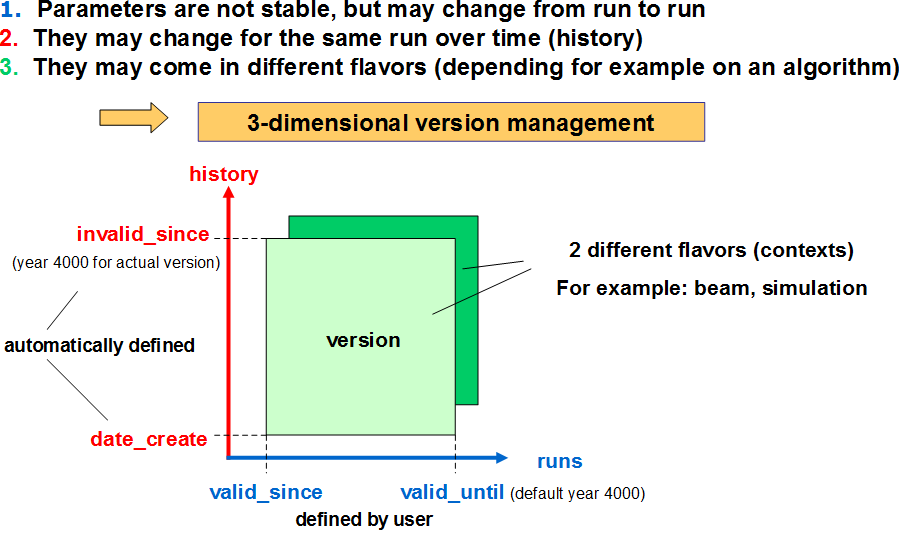
\includegraphics[scale=0.50]{hydra2_ora_versionmanagement_1.png}
  \caption[Parameters for the version management]{Parameters for the version management}
  \label{fig:oraVersionmanagementParameters}
\end{figure}

A parameter or parameter set has 5 variables in Oracle for the version management:\\
\begin{tabular}{|l|l|}
  \hline
  \cellcolor{lightgray} \textit{Variable} & \cellcolor{lightgray} \textit{Description}\\
  \hline
  valid\_since                    & First date when the entry is valid.\\
  \hline
  \multirow{2}{*}{valid\_until}   & Last date when the entry is still valid.\\
                                  & (High date ``01-JAN-4000 00:00:00`` for last version actually still valid)\\
  \hline
  date\_create                    & Date when a version is inserted\\
  \hline
  \multirow{2}{*}{invalid\_since} & Date when the entry is replaced by a new or better version and therefore gets invalid.\\
                                  & (High date ``01-JAN-4000 00:00:00`` for valid version, historic dates for invalid ones)\\
  \hline
  context\_id                     & Identifier of the parameter context\\
  \hline
\end{tabular}\\

Valid\_since and valid\_until define a time range on the runs axis. They are defined by the user in the WebDB validation form.\\
Date\_create and invalid\_since define a time range on the history axis and are set automatically by the validation interface.\\

Additionally the author and a description is stored for each version.

\paragraph{Example:} ~\\
Figure \ref{fig:oraVersionmanagementFinding1}: A user validates a version 1 of for example calibration parameters at the 
beginning of a beam time starting at valid\_since\_1. He does not specify an end of the time range, but leaves it open. The 
program sets the end to the January 1st  in year 4000.\\ 
The analysis of every new run will now get the version 1.\\
After some time, after for example new pedestals have been taken, he validates a new version 2, starting at valid\_since\_2, 
and again open-end.\\
The web interface first changes the value of the invalid\_since column in the version 1 record from year 4000 to the actual 
date minus one second. Then it inserts the version 1 again with the time range ending at valid\_until\_1. This is one second 
less than the new valid\_since of version 2. Then it inserts the new version 2. This leads to three rectangles which do not 
overlap.\\
Now every new run is initialized with version 2.
\begin{figure}[\htb]
  \centering
  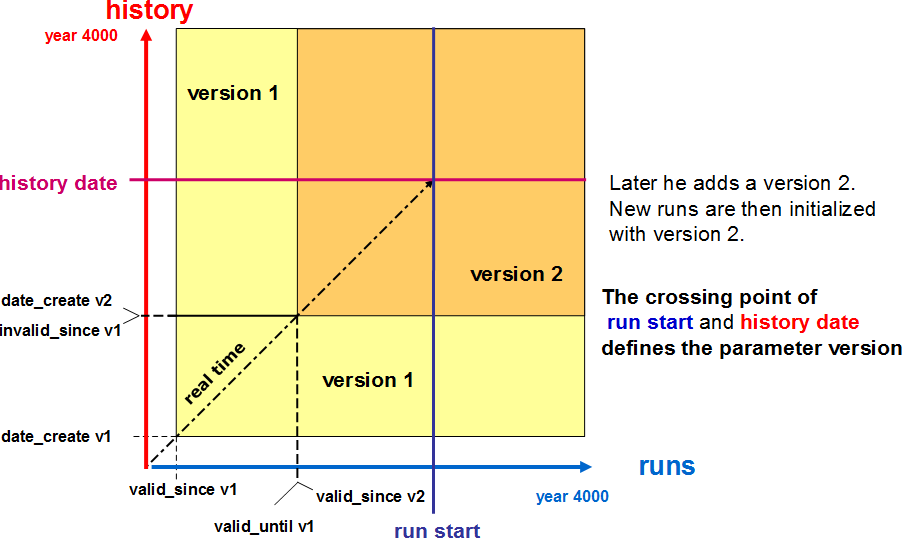
\includegraphics[scale=0.50]{hydra2_ora_versionmanagement_2.png}
  \caption[Finding the version (1)]{Finding the version (1)}
  \label{fig:oraVersionmanagementFinding1}
\end{figure}

Figure \ref{fig:oraVersionmanagementFinding2}: After a re-calibration maybe after the beam time, the user comes up with new 
version 3 and 4, which replace the old ones.
\begin{figure}[\htb]
  \centering
  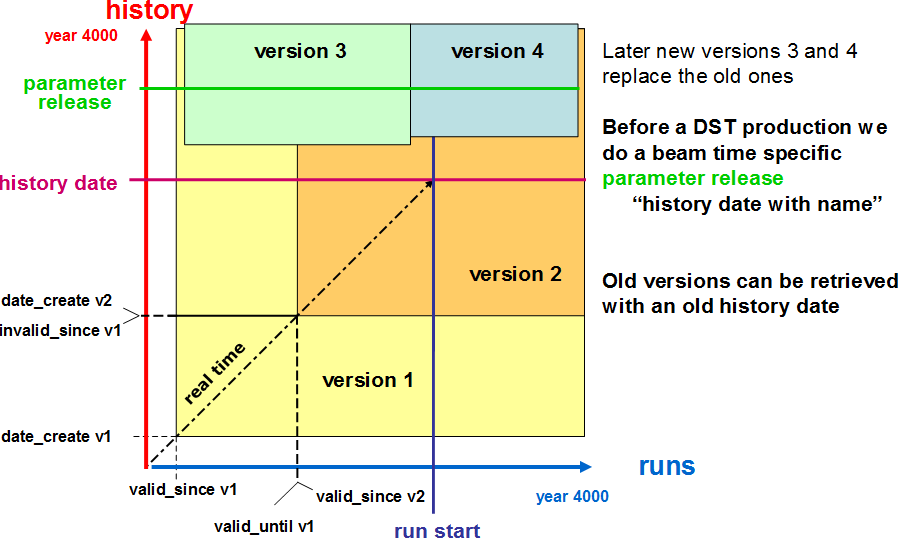
\includegraphics[scale=0.50]{hydra2_ora_versionmanagement_3.png}
  \caption[Finding the version(2)]{Finding the version(2)}
  \label{fig:oraVersionmanagementFinding2}
\end{figure}

Not all parameter containers are independent. Therefore we create before a DST production a beam time specific parameter release, 
which is a history date with a name stored in the data base. By default the last parameter release is used for initialization. 
But the user can overrule this in the macro and set any history date.
\clearpage


\section[The WebDB Site]{The WebDB Site} \label{sec:oraWebdbSite}

All web interfaces are accessible from the WebDB Site after login.
\paragraph{Login:} ~\\
Direct link:\\
\verb+    http://webdb.gsi.de/pls/hades_webdb/hxsite.main+\\
Click on Login button to get the login form.\\

From the HADES web page:\\
 $\Rightarrow$ internal $\Rightarrow$ WebDB\\
The login form pops up.\\

Login as user (not case sensitive)\\
\begin{tabular}{l p{14cm}}
\textbf{hades}     & This user has read-only access to most of the applications and can insert entries into the 
                   beam time log book and the shift plan of a beam time. \\
\textbf{xxx\_oper} & Each detector and the DAQ have specific access accounts to insert and change data via forms, 
                   mdc\_oper for example can validate MDC parameters. \\
\end{tabular}\\

Fig.~\ref{fig:oraWebdbSite} shows the page after login.\\
All applications are stored in a tree-like folder structure. The navigation on the left side shows the links to the folders 
accessible by the user, the right side their content (here the content of the ROOT folder).

\begin{figure}[\htb]
  \centering
  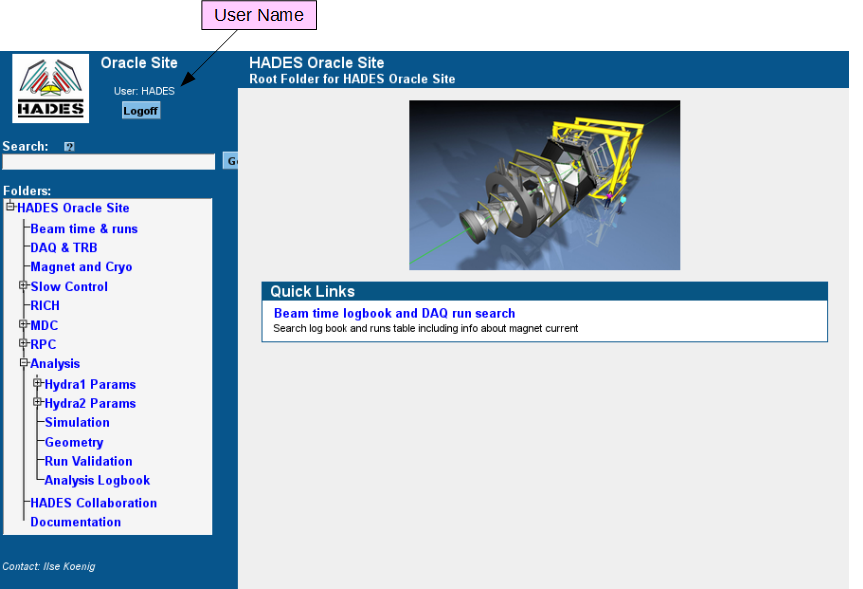
\includegraphics[scale=0.50]{hydra2_ora_webdbsite.png}
  \caption[The WebDB Site]{The WebDB Site}
  \label{fig:oraWebdbSite}
\end{figure}

\paragraph{Tip:} In the upper left part you can see the user name. The web browser typically keeps the http authentification 
after logout. When you switch from user hades to xxx\_oper you might still be logged in as user hades. You will not 
see some detector specific folders or applications or get error messages (``Insufficient privileges'').\\
Either clear the private cache or kill all browser windows and start again from a new one.  

The next pages show some WebDB applications useful for analysis users (\textbf{\color{red}Status at 20-JUL-2015)}.


\section[Experiments]{Experiments} \label{sec:oraExperiments}

The most central table in Oracle is the one for experiments. It defines a time range for DAQ runs and simulation reference
runs, beam time logbook entries, shift plans and many more.\\

The application ``\textbf{Experiment info}`` in the folder ``\textbf{Beamtime \& runs}'' allows to search for experiments. 
Fig.~\ref{fig:oraFormExperiments} shows the form\footnote{Some applications are shown in the full window. The icon link 
``Back to folder`` leads back the the folder page with the navigation bar on the left side.} and 
fig.~\ref{fig:oraExperiments} the corresponding result. The yellow lines shows the beam times and detector tests in the 
HADES cave, the blue ones the simulation projects (location VIRTUAL) and the red line a beam time outside 
GSI\footnote{To use the beam time logbook a beam time must be defined.}.\\
The time range begin - end and the location is used to get the lists of runs in the analysis interface.

\begin{figure}[\htb]
  \centering
  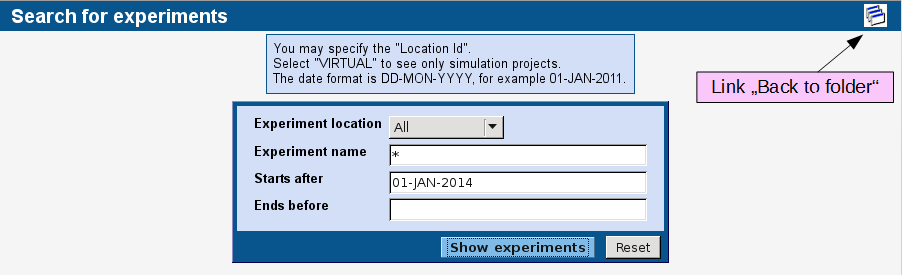
\includegraphics[scale=0.65]{hydra2_ora_form_experiments.png}
  \caption[Form to search for experiments]{Form to search for experiments}
  \label{fig:oraFormExperiments}
\end{figure}

\begin{figure}[\htb]
  \centering
  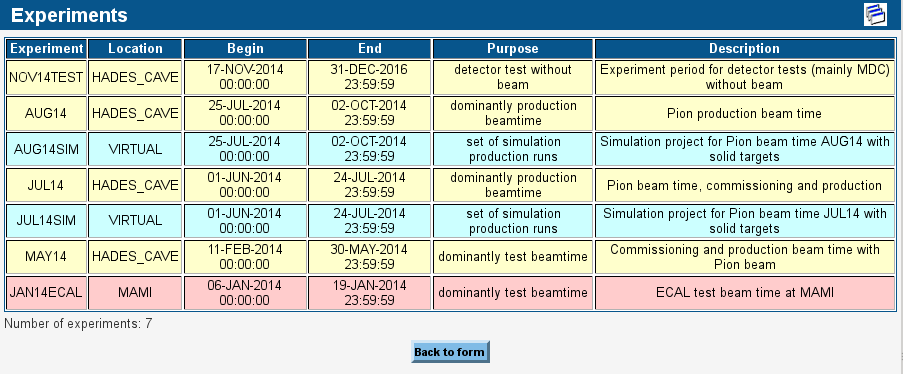
\includegraphics[scale=0.65]{hydra2_ora_experiments.png}
  \caption[Experiments]{List of experiments in specified time range}
  \label{fig:oraExperiments}
\end{figure}


\subsection[DAQ runs]{DAQ runs} \label{sec:oraDaqRuns}
DAQ runs are stored in Oracle online by Perl scripts and can be shown in the beam time logbook. Not shown there are the list 
of files (one for each event builder) belonging to the run.\\
The master event builder defines the run id (time of the first event in seconds since 01-JAN-1970 minus $1.2\times10^9$) common 
for all event builder files. The smallest start time of all files with non-zero events is stored as start time of this run. 
All files with the same run id use this start time for the initialization of the analysis parameters.\\ 
The common run type is defined by the file prefix, for example run type BEAM by prefix \verb+be+, COSMIC by \verb+co+.\\

The application ``\textbf{Charts of beam time and run statistics}`` in folder ``\textbf{Beamtime \&runs}'' (topic Monitoring) allows to 
show the statistic for beam time runs and the corresponding event builder files.\\
After selecting a beam time one gets the form shown in the upper part of fig.~\ref{fig:oraRunStatistic}. See the HELP for 
instructions to filter the data and to produce different bar charts (for example number of runs, number of events, \ldots).\\
The lower part in the figure shows the result of the selection grouped by day.\\
The color indicates the mean magnet current (always averaged over the time range of one bar).\\
If one clicks on the day link one would get the 
results by hour and if one clicks there on an hour link one gets the list of files with non-zero events. 
Fig.~\ref{fig:oraDaqFiles} shows an example.
\begin{figure}[\htb]
  \centering
  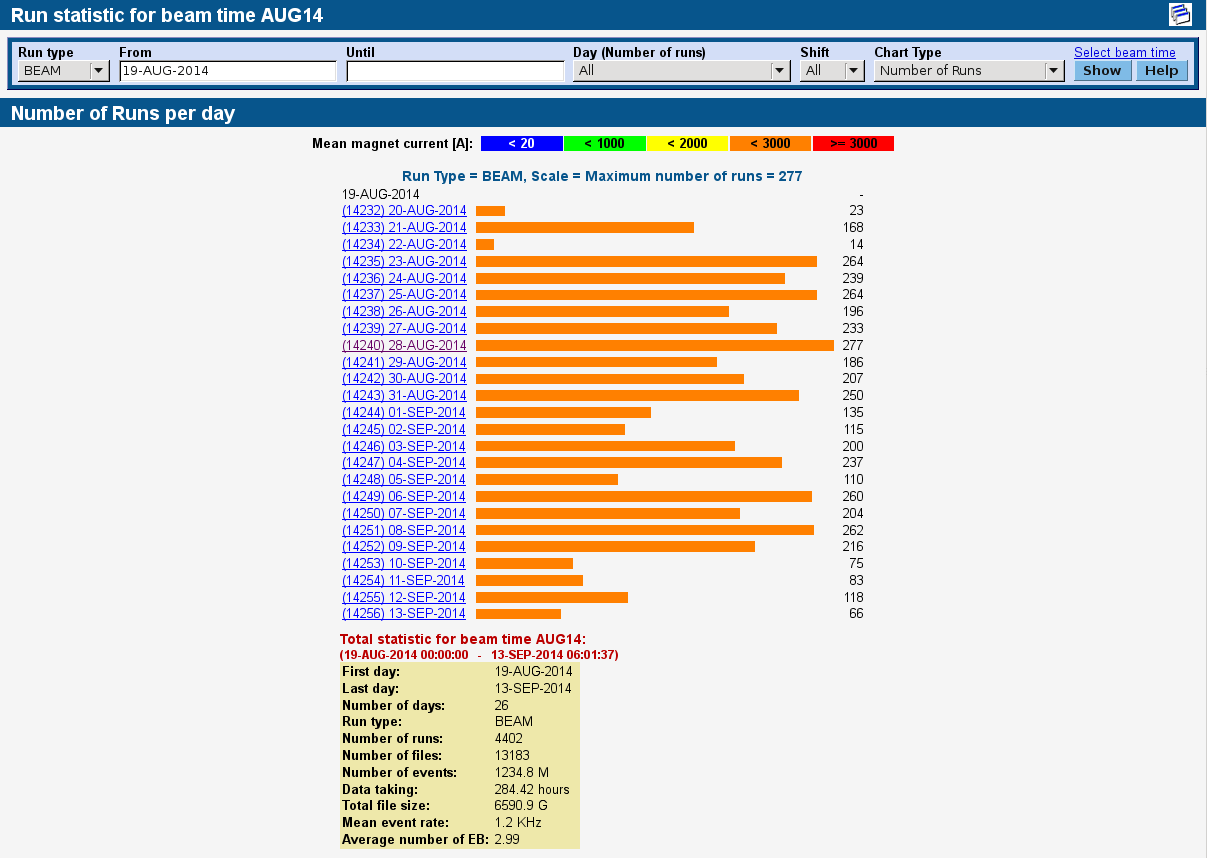
\includegraphics[scale=0.50]{hydra2_ora_runstatistic.png}
  \caption[Beam time and run statistic]{Beam time and run statistic}
  \label{fig:oraRunStatistic}
\end{figure}

\begin{figure}[\htb]
  \centering
  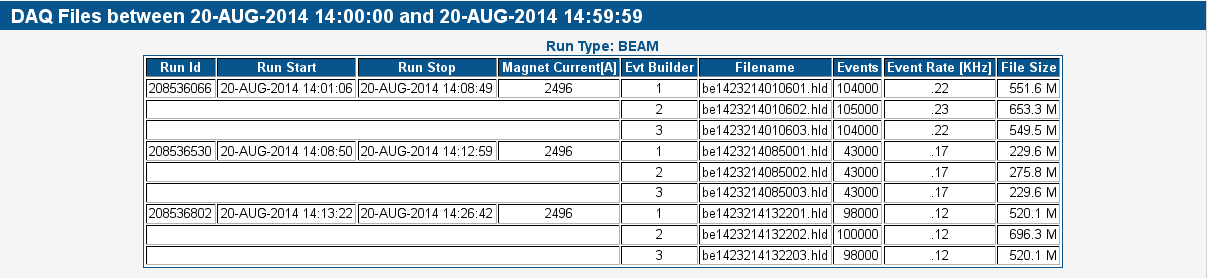
\includegraphics[scale=0.50]{hydra2_ora_runstatistic_files.png}
  \caption[DAQ runs and files]{DAQ runs and files}
  \label{fig:oraDaqFiles}
\end{figure}


\subsection[Simulation projects and reference runs]{Simulation projects and reference runs} \label{sec:oraSimulProjects}

The version management in Oracle is based on time ranges. Each DAQ run has a start time and this time stamp (together with 
the history date and the context) defines the version used for the initialization of this run. Runs are taken in consecutive 
order and have no time overlap.\\
On the other hand simulations are done in parallel for different beam times or proposals for future experiments and the real 
start time is not a good ordering parameter.\\
To use the same tables/views and interfaces in Oracle it was necessary to give simulation runs artificial timestamps and to group 
them in projects and sub-projects.\footnote{The additional grouping in generations was discarded for simulation 
projects since 2010.}\\

A \textbf{simulation project} is typically a simulation for a beam time (example APR12SIM) and has also the same time range. 
But to do simulations for future experiments, for example to simulate the replacement of the Shower detector by the ECAL, 
and to store dedicated geometry setups for it, some projects have been added with intermediate time ranges (example ECAL13SIM).
\newpage

Each project contains \textbf{sub-projects} with fixed
\begin{itemize}
  \setlength{\itemsep}{0pt}    
  \item projectile + target system
  \item projectile energy
  \item field setting
  \item target
\end{itemize}
Each sub-project has an artificial time range of one day. It has at least one \textbf{reference run} with a descriptive 
name and a run id easy to remember. The first reference run typically starts at midnight and has a duration of only one 
second.\\ 
The run id is used in the analysis as reference run for the initialization of parameter containers, while the name is 
used in the HGeant2 configuration file to read the geometry (see \ref{sec:geomGeaini}).\\ 

Fig.~\ref{fig:oraSimulProjects} shows the WebDB application in folder ``\textbf{Analysis $\Rightarrow$ Simulation}'' which allows 
to get the list of reference runs for a selected simulation project, here as example for the simulations for the Pion 
beam time in August 2014. 
\begin{figure}[\htb]
  \centering
  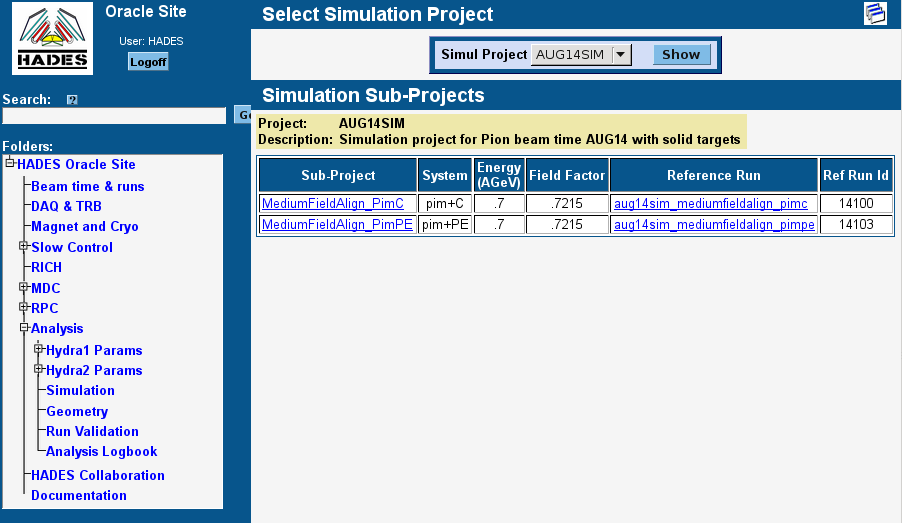
\includegraphics[scale=0.65]{hydra2_ora_simulprojects.png}
  \caption[Simulation sub-projects and reference runs]{Simulation sub-projects and reference runs}
  \label{fig:oraSimulProjects}
\end{figure}

If people validate parameters for simulation they use links in pop-up windows showing the projects and sub-projects names. 
A click on the link adds the corresponding time in the form, time begin for valid\_since, time end for valid\_until.\\
Also in the public interface typically only the names of the reference runs are visible, not the time stamps.\\  

Because the time stamps are so artificial and the rules hard to remember, a WebDB interface was developed to make it 
more comfortable to add projects and sub-projects and to avoid mistakes. The link is in the same folder but one needs 
to login as a special user to execute it.


\section[The WebDB folder Hydra2 Params]{The WebDB folder Hydra2 Params} 
\label{sec:oraFolderHydra2Params}

For the change from Hydra1 to Hydra2 a major revision of the Oracle production accounts was done in 2009. Backward 
compatibility was not required. Many new accounts  were created with partially different table design. Only the last 
versions of the parameters were copied into these tables and validated since 01-JAN-2010. The Hydra2 analysis interface cannot 
read Hydra1 parameter containers and vice versa.\\
Many web interfaces were cleaned and modernized (new framework with CSS and Javascript). The old Hydra1 web interfaces 
were not touched and still use the old layout.\\

The folder ``\textbf{Analysis $\Rightarrow$ Hydra2 Params}'' (Fig.~\ref{fig:oraFolderHydra2Params}) contains the applications 
related to parameter containers in Hydra2. It contains also sub-folders for tree- and condition-style parameter containers.

\begin{figure}[\htb]
  \centering
  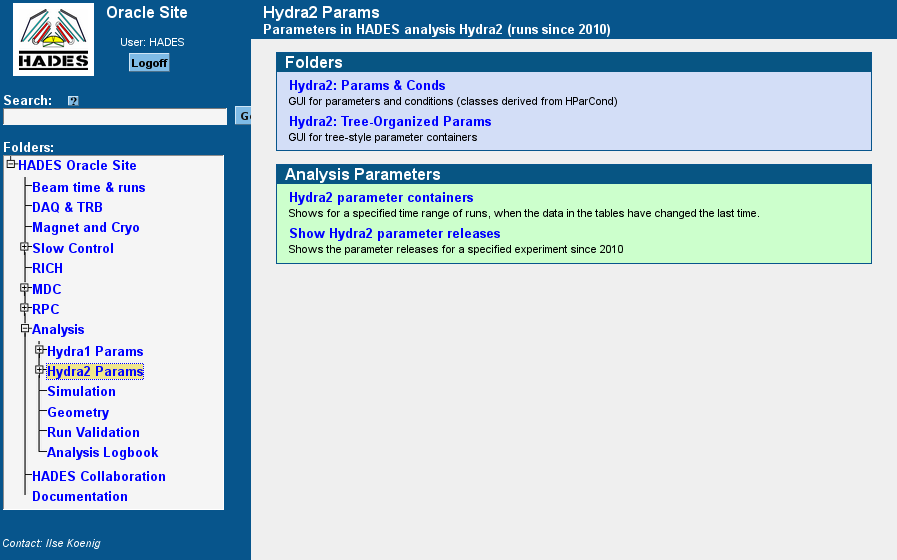
\includegraphics[scale=0.65]{hydra2_ora_folder_hydra2_params.png}
  \caption[The WebDB folder Analysis $\Rightarrow$ Hydra2 Params]{The WebDB folder Analysis $\Rightarrow$ Hydra2 Params}
  \label{fig:oraFolderHydra2Params}
\end{figure}


\subsection[Parameter releases]{Parameter releases} \label{sec:oraParameterReleases}

Fig.~\ref{fig:oraParameterReleases} shows an example of the application ``\textbf{Show Hydra2 parameter releases}''.\\
As first step one fills the form in the upper part and selects one or more beam times and/or simulation projects. If one 
then clicks on \verb+Show+ one gets the list of all parameter releases. The green line shows the current one, which would 
be used for initialization if no history date it set explicitly.  

\begin{figure}[\htb]
  \centering
  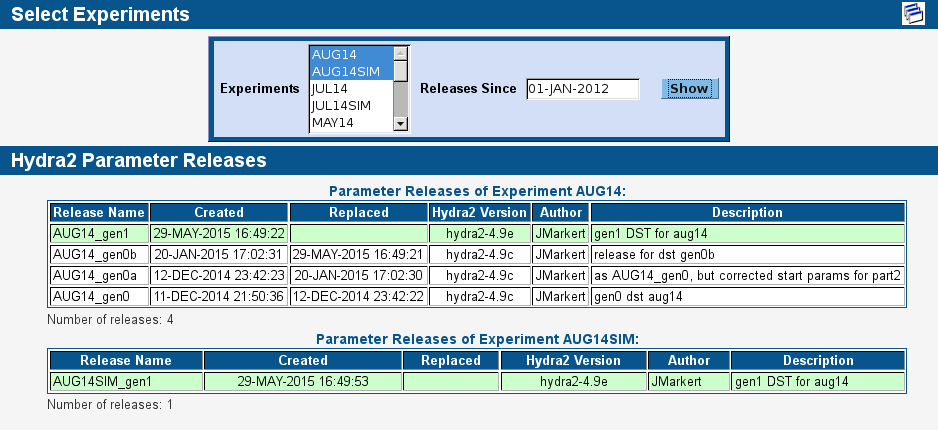
\includegraphics[scale=0.62]{hydra2_ora_parameter_releases.png}
  \caption[Hydra2 parameter releases]{Hydra2 parameter releases}
  \label{fig:oraParameterReleases}
\end{figure}


\subsection[Overview of parameter containers]{Overview of parameter containers} \label{sec:oraParameterContainers}

Fig.~\ref{fig:oraHydra2Params} shows an example of the application ``\textbf{Hydra2 parameter containers}''.\\
For a selected beam time it lists all parameter containers (still missing: geometry parameter containers) with the 
time stamp of the last change, in red the ones which changed since the last parameter release\footnote{In the entrance form one 
may set a date to highlight all later changes. This might be usesful if one created a parameter ROOT file once and wants to 
see which parameters changed meanwhile.}.

\begin{figure}[\htb]
  \centering
  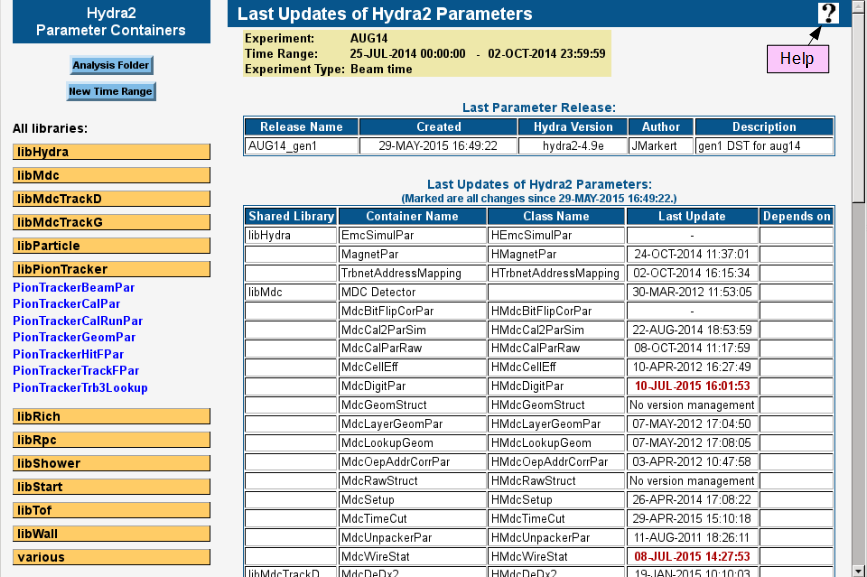
\includegraphics[scale=0.62]{hydra2_ora_hydra2_params.png}
  \caption[Hydra2 parameter containers overview]{Hydra2 parameter containers overview}
  \label{fig:oraHydra2Params}
\end{figure}

The navigation bar on the left side provides access to the parameter containers grouped by the shared libraries. Click on a 
shared library to see the links to the data pages for the parameter containers in this library. 


\section[Condition-style parameter containers]{Condition-style parameter containers} \label{sec:oraCondStyle}

\begin{figure}[\htb]
  \centering
  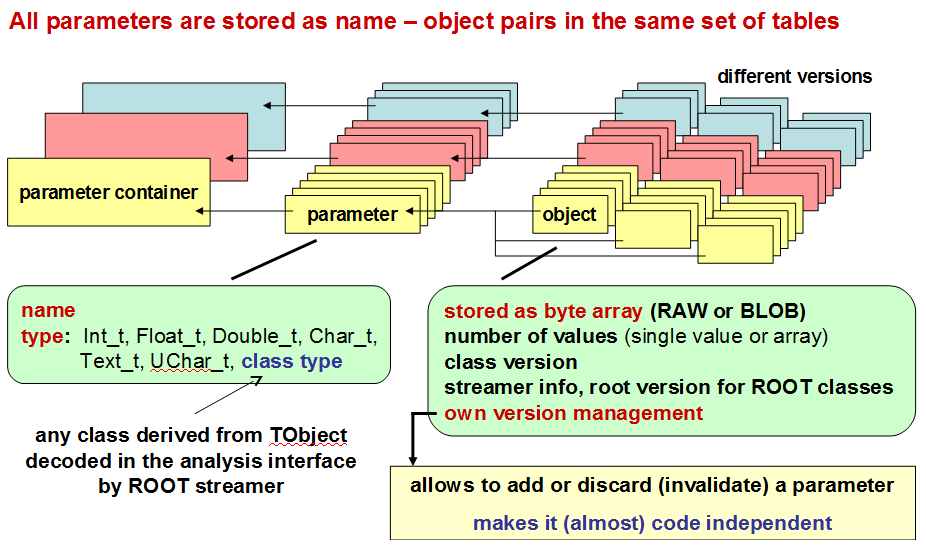
\includegraphics[scale=0.50]{hydra2_ora_hparcond.png}
  \caption[Storage of condition-style parameter containers]{Storage of condition-style parameter containers}
  \label{fig:oraCondStyleStorage}
\end{figure}

Each parameter belongs to a parameter container, has a name and a type. Possible types are the basic ROOT c-types, 
but also any class derived from TObject.\\
Different data objects (= different versions) exist for each parameter. The data are stored as byte array either in a RAW 
column for single number values and small arrays or in a binary large object (BLOB). Also stored is the number of values and for 
classes the class version, for ROOT classes additionally the streamer info and the ROOT version for backward compatibility. 
Basic types can be decoded in the web interface, classes only in the c++ interface with the ROOT streamer.\\

Each data object has its own version management, which allows to add a new parameter or to discard an old parameter no 
longer needed without any change of the other parameters. The analysis interface reads all parameters valid for the 
specified run and history date and stores them in a list. The parameter container takes from the list only the parameters 
(= data members) in the current class version. This makes the interface code independent.

\subsection[Search for parameter sets]{Search for parameter sets} \label{sec:oraSearchParamSets}

Fig.~\ref{fig:oraFolderParamaAndConds} shows the applications in the folder 
``\textbf{Hydra2 Params $\Rightarrow$ Params \& Conds}'' for condition-style parameter containers.

\begin{figure}[\htb]
  \centering
  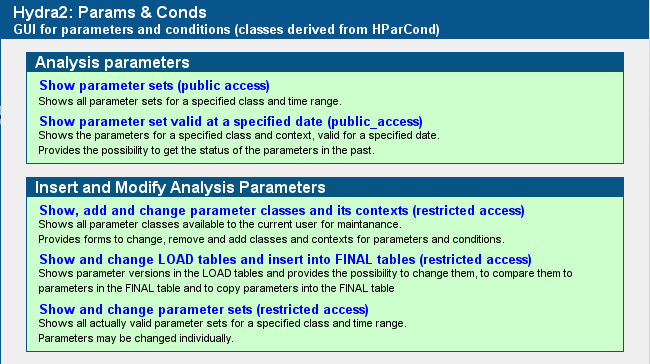
\includegraphics[scale=0.70]{hydra2_ora_folder_paramsandconds.png}
  \caption[Folder Hydra2 Params $\Rightarrow$ Params \& Conds]{Folder Hydra2 Params $\Rightarrow$ Params \& Conds}
  \label{fig:oraFolderParamaAndConds}
\end{figure}

The application ``\textbf{Show parameter sets}'' allows to search for the parameter sets of a selected parameter container  and 
experiment. Fig.~\ref{fig:oraHMdcDigiParSets} shows the result for the parameter container \verb+MdcDigiPar+ and beam time 
AUG14.\footnote{For event embedding simulation parameters must be also validated for beam runs.} \\
The program searches for all valid parameters in the beam time range. If one or more parameters change in this time range one 
will see more than one set. The time range of one set is the maximum of the valid\_since of the parameters and the minimum 
of all valid\_until.\\

\begin{figure}[\htb]
  \centering
  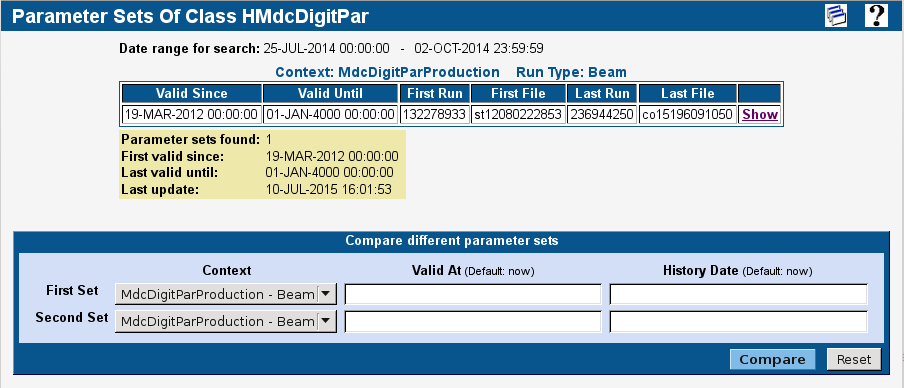
\includegraphics[scale=0.62]{hydra2_ora_hmdcdigipar_sets.png}
  \caption[Parameters sets of class HMdcDigiPar]{Parameters sets of class HMdcDigiPar}
  \label{fig:oraHMdcDigiParSets}
\end{figure}

The link \verb+Show+ displays the valid data, the time stamps of the version management and a link to display the comment 
(fig.~\ref{fig:oraHMdcDigiParData}). Some columns may be sorted, here for \verb+Date Create+.

\begin{figure}[\htb]
  \centering
  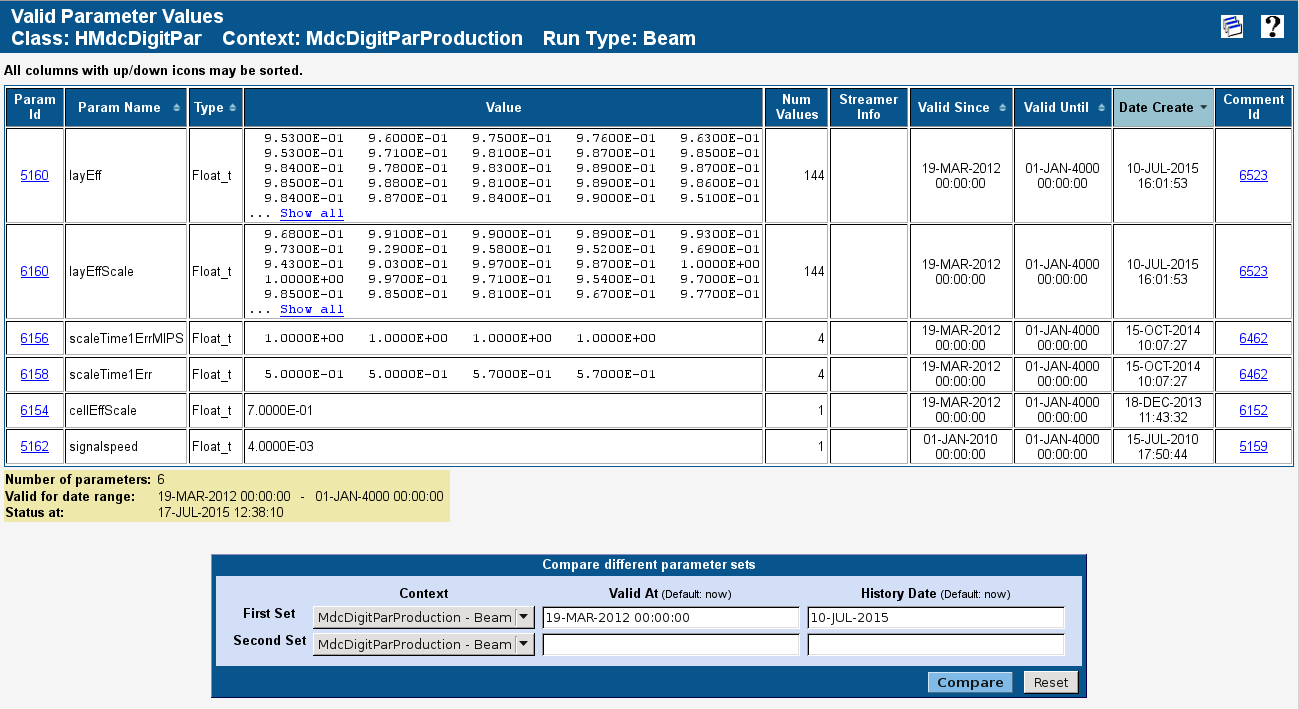
\includegraphics[scale=0.50]{hydra2_ora_hmdcdigipar_data.png}
  \caption[Parameters of class HMdcDigiPar]{Parameters of class HMdcDigiPar}
  \label{fig:oraHMdcDigiParData}
\end{figure}

The form in fig.~\ref{fig:oraHMdcDigiParData} allows to compare parameter sets. In this example one will see the 
differences of the data compared to the historic data valid before the last validation at \verb+10-JUL-2015 16:01:53+ (fig.~\ref{fig:oraHMdcDigiParComparison}).

\begin{figure}[\htb]
  \centering
  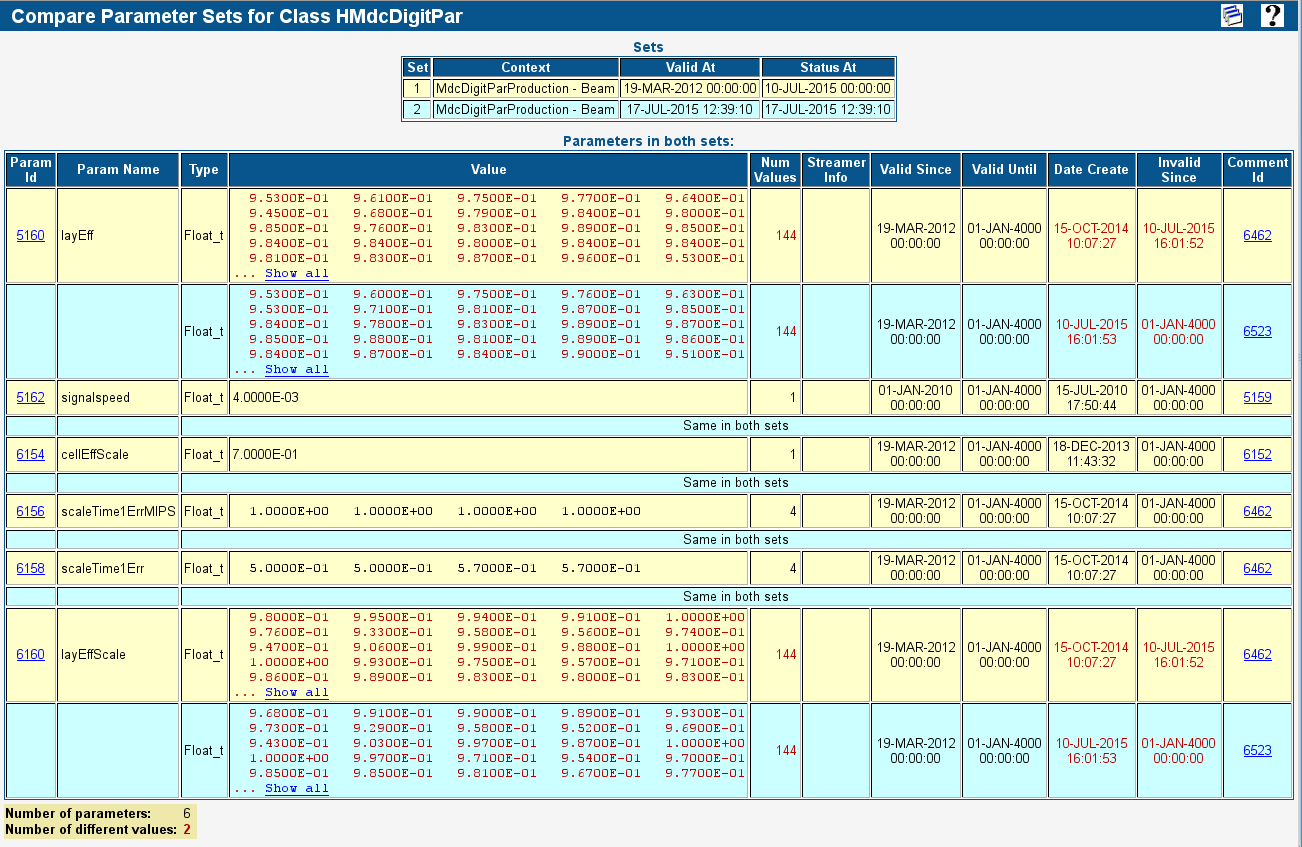
\includegraphics[scale=0.50]{hydra2_ora_hmdcdigipar_comparison.png}
  \caption[Result of comparison]{Result of comparison}
  \label{fig:oraHMdcDigiParComparison}
\end{figure}
\clearpage

In this example the first set is the historic one, the second the actual valid set. As \verb+Valid At+ for the first set, 
one chooses the last \verb+Valid Since+ of all parameters. As \verb+History Date+ one puts a time stamp at least one 
second earlier as the last \verb+Date Create+ (if omitted the time part is set to 00:00:00).\\
Fig.~\ref{fig:oraHMdcDigiParComparison} shows the result. The differences are shown in red. As expected two 
parameters were changed.\\

For event embedding in the analysis it is essential that the parameters needed by the digitizer are the same for beam  
and simulation runs. To check this one can compare the parameters by choosing different contexts in the form, but 
the same \verb+Valid At+ and \verb+History Date+. The parameter values should be the same, only the \verb+Date Create+ 
is typically different, because two validations, one for beam and one for simulation runs were done.

\subsection[Adding a new class]{Adding a new class}

The folder ``\textbf{Hydra2 Params $\Rightarrow$ Params \& Conds}`` contains also the non-public applications to store, validate 
and change condition-style parameter containers.\\
The privilege to manage the data is granted by library. For example the account TOF\_OPER can manage parameter containers in 
libTof (and also libStart). The drop-down menus only show classes or libraries the user logged in can manage.

If one creates a new condition-style parameter container in Hydra2 one must add this class and its context in Oracle before 
one can write the parameters into the database.
The application ``\textbf{Show, add and change parameter classes and its contexts (restricted access)}'' lists all parameter 
containers the user can manage and below a button \verb+Add New Class+. It leads to a form where one selects the library, 
specifies the class name, the name of the parameter container, the standard context name and the run type(s) for the
context (beam runs, simulations runs or both).

In the list of parameter containers it shows up as a red line. This means, one can write the parameters to Oracle but 
not validate them (no link). First Jochen Markert or Ilse Koenig must \textbf{confirm} the new class. As long as not validated 
the class and the data can be deleted from Oracle, once validated this is not allowed anymore (and very complicated).
The confirmation is a kind of security check to avoid the storage of parameter containers not accepted in Hydra2 and code not 
committed to SVN.

\subsection[Parameter validation]{Parameter validation} \label{sec:oraParameterValidation}

If one writes a condition-style parameter container into Oracle, the data are \textbf{not} stored in the final tables but 
in intermediate so-called LOAD tables. Here parameters can be changed, even new parameters added. After validation the 
data can be removed from the LOAD tables.\footnote{One should only keep standard versions in the LOAD tables, which one must validate more often 
for different time ranges, for example different versions of MagnetPar with the standard current settings. All others should 
be deleted to avoid mistakes.}

\begin{figure}[\htb]
  \centering
  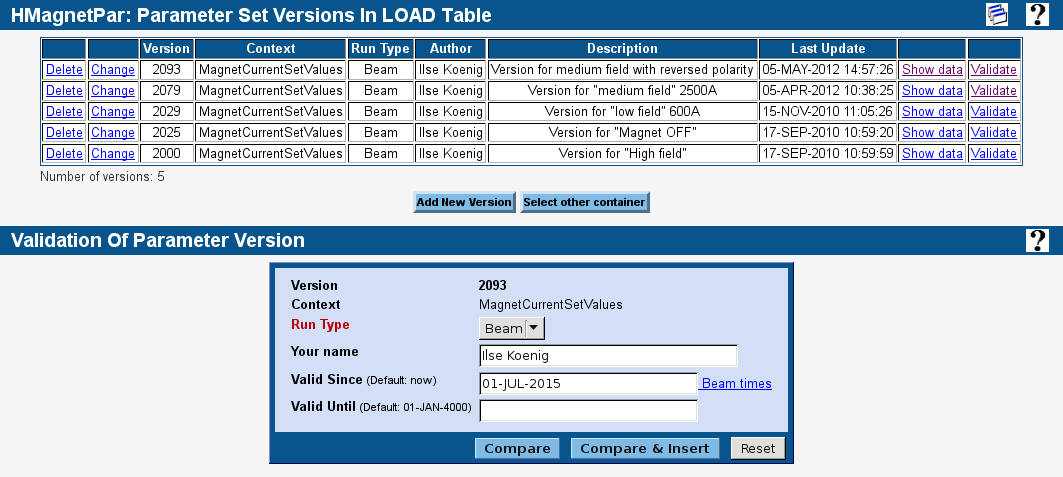
\includegraphics[scale=0.60]{hydra2_ora_form_validate.png}
  \caption[Show and validate parameters in the LOAD tables]{Show and validate parameters in the LOAD tables}
  \label{fig:oraFormValidate}
\end{figure}

The application ``\textbf{Show and change LOAD tables and insert into FINAL tables}'' shows all sets in the LOAD tables for  
a selected parameter container, in the upper part of figure~\ref{fig:oraFormValidate} as example for the parameter 
container MagnetPar. The link \verb+Validate+ of the uppermost version leads to the validation form below. Here one chooses 
the run type (Beam or Simul) and specifies the validity time range.\\
The link \verb+Beam times+ lists all beam times with their begin and end dates as links. If one clicks on a link the 
corresponding date is transferred to the form field.\\
For more details read the \verb+Help+.\\

Figure~\ref{fig:oraValidate} shows the result if one clicks on the button \verb+Compare & Insert+. The program loops over 
all parameters, for each compares the new value with the value(s) valid in the specified time range and shows a preview of 
all changes.\\
Figure~\ref{fig:oraHelpValidate} on page~\pageref{fig:oraHelpValidate} shows the corresponding \verb+Help+ page with a 
detailed description.

\begin{figure}[\htb]
  \centering
  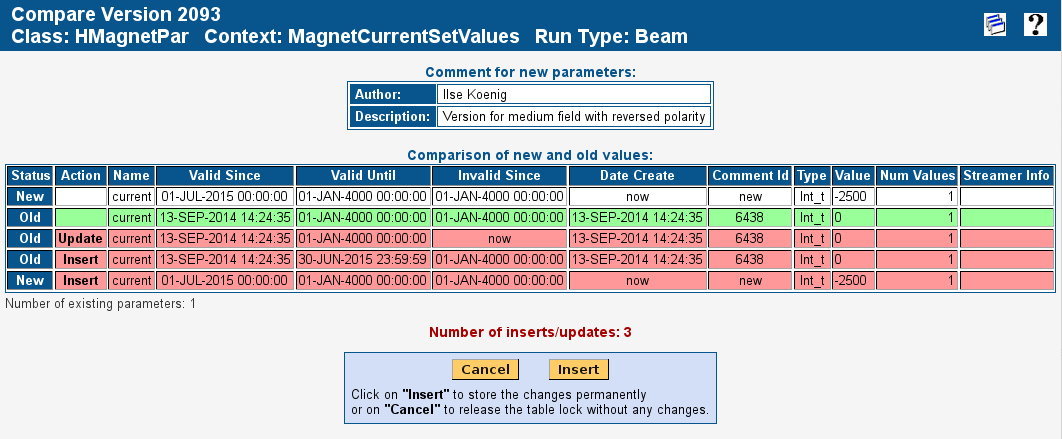
\includegraphics[scale=0.60]{hydra2_ora_validate.png}
  \caption[Preview of validation for condition-style parameter containers]
          {Preview of validation for condition-style parameter containers}
  \label{fig:oraValidate}
\end{figure}

\begin{figure}[\htb]
  \centering
  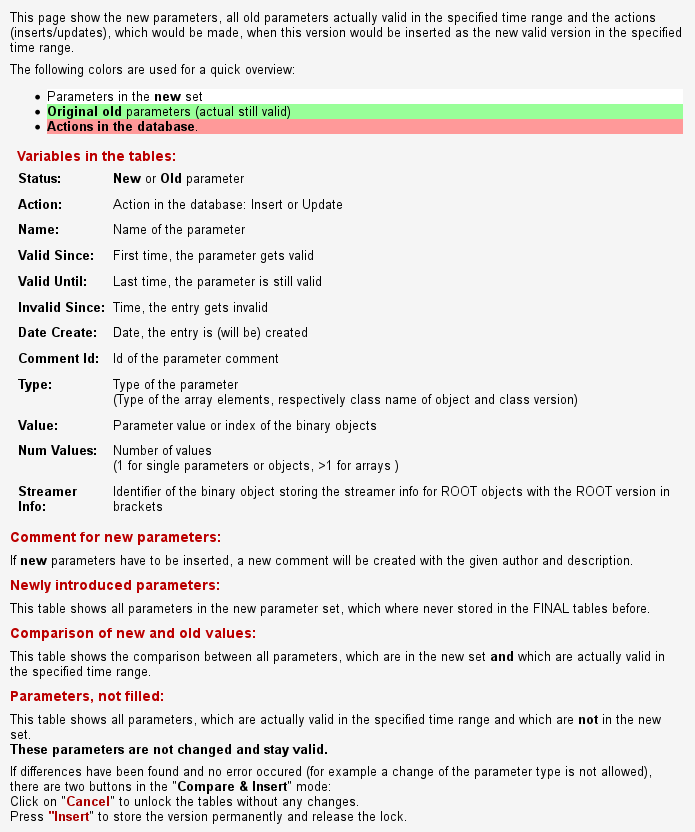
\includegraphics[scale=0.80]{hydra2_ora_help_validate.png}
  \caption[Help page of validation preview for condition-style parameter containers]
          {Help page of validation preview for condition-style parameter containers}
  \label{fig:oraHelpValidate}
\end{figure}

\subsubsection{How to get a valid parameter set into the LOAD tables}

The application ``\textbf{Show and change parameter sets}'' does not only allow to change the validity time ranges of valid 
parameter sets or individual parameters (see \verb+Help+ for details) but also provides a form to get a valid set into 
the LOAD tables without the need to run a macro in Hydra2.\\

Recipe:\\
In the form select the parameter container and the beam time or simulation project (or specify a longer time range). Click 
on the button \verb+Show Sets+.\\
This shows all valid parameter sets. Click on the \verb+Show+ link of the version you want to copy.\\
It shows the data of all parameters in this set and below a form to copy the data. Specify the author and the comment 
and click on \verb+Copy Set+.

\section[Tree-style parameter containers]{Tree-style parameter containers} \label{sec:oraTreeStyle}

Although the storage of tree-style parameters is completely different the WebDB interface is quite similar to condition-style 
parameter containers.\\
The main difference comes from the fact, that the analysis interface creates a version and writes the data of this version 
directly into the final tables.\\
The values are stored as rows, each consisting of the version id, an address identifier (for example a cell id) and the 
values of all data members in separate columns (similar to the ASCII file). All rows with the same version id 
build one parameter set.\\
The validation interface validates the version number. It simply compares the version numbers with the ones actually valid in 
the specified time range. The parameters themselves are \textbf{not} compared.\\
 
All interfaces are in the folder \textbf{Hydra2 Params $\Rightarrow$ Tree-Organized Params}.
\clearpage

\section[Geometry]{Geometry} \label{sec:oraGeometry}

The WebDB folder Geometry contains various public applications to display the geometry information (valid versions, tree of detector 
volumes and volume, media, hit definitions) and non-public applications for storage and changes.
 
Fig.~\ref{fig:oraGeometrySets} shows as example the result of the application ``\textbf{Show geometry}'' after selecting 
the beam time APR12 in the entry form (not shown). It shows all versions validated for real runs in this time range.
\begin{figure}[\htb]
  \centering
  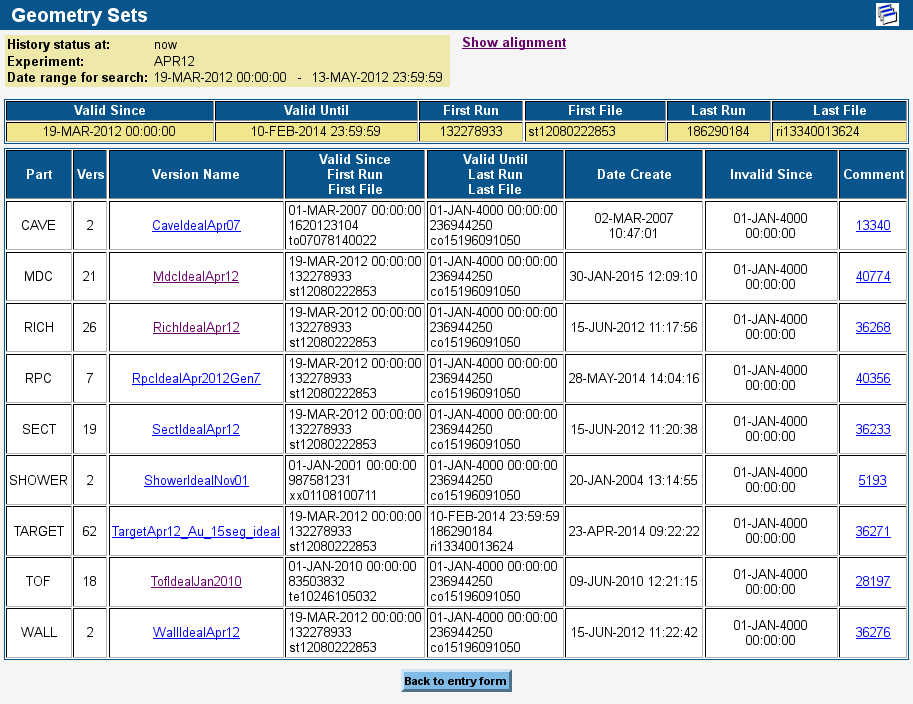
\includegraphics[scale=0.60]{hydra2_ora_geometry_sets.png}
  \caption[Geometry set for beam time APR12]
          {Geometry set for beam time APR12}
  \label{fig:oraGeometrySets}
\end{figure}

If one clicks on the link of a version name one gets the full geometry tree of this version. Fig.~\ref{fig:oraMdcGeomTree} 
shows on the left side for example the MDC geometry tree. The link of the volume name pops up a separate window and shows 
the volume definition, here on the right side for the volume DR1M1, the MDC plane 1 mother volume in sector 1.
\begin{figure}[\htb]
  \centering
  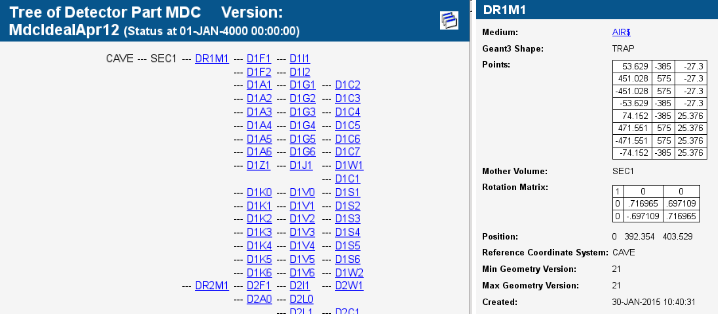
\includegraphics[scale=0.80]{hydra2_ora_mdc_geomtree.png}
  \caption[MDC geometry tree of version MdcIdealApr12]
          {Mdc geometry tree of version MdcIdealApr12}
  \label{fig:oraMdcGeomTree}
\end{figure}

If one would instead select the simulation project APR12 in the entry form of the application one would see two sets for 
the two reference runs apr12sim\_mediumfieldideal\_auau with ideal geometry and apr12sim\_mediumfieldalign\_auau with the 
alignment geometry. Each set also includes the valid versions of the coils, the frames and the Start detector (not needed 
for the APR12 analysis). Instead of the link \textbf{Show alignment} one would see the link \textbf{Show hit definition}.\\

Fig.~\ref{fig:oraAlignment} shows the corresponding alignment versions for beam time APR12.
\begin{figure}[\htb]
  \centering
  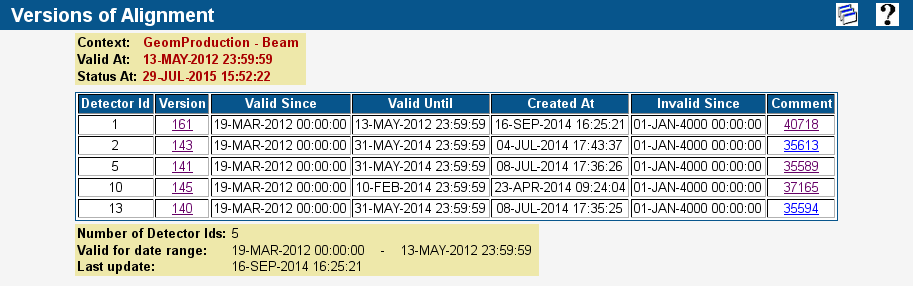
\includegraphics[scale=0.60]{hydra2_ora_alignment.png}
  \caption[Alignment for beam time APR12]
          {Alignment for beam time APR12}
  \label{fig:oraAlignment}
\end{figure} ~\\
Unfortunately the generic interface does not allow to display the detector by name, but only by id:\\
1: TOF, 2: MDC, 5: Shower, 8: Start, 10: Target, 11: Forward Wall, 13: RPC, 14: EMC\\ 

The link of the version number shows the alignment LAB-transformation, for example in fig.~\ref{fig:oraTargetAlignment} 
the 15 target positions of the segmented Gold target.
\begin{figure}[\htb]
  \centering
  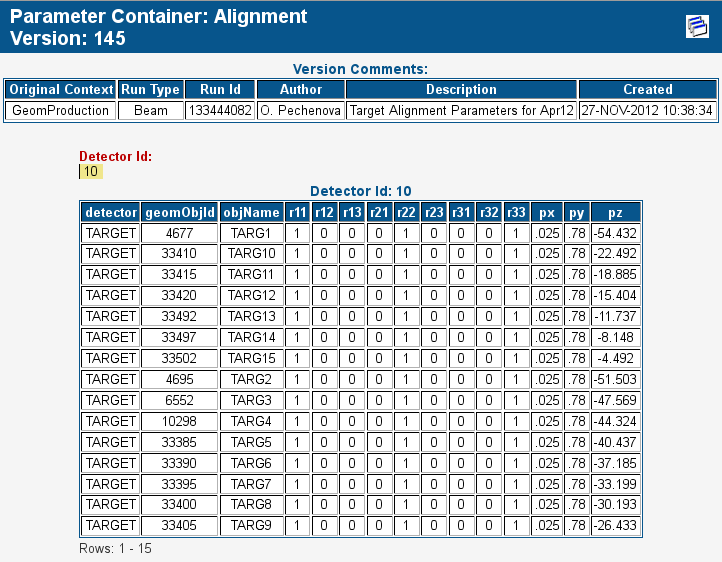
\includegraphics[scale=0.60]{hydra2_ora_target_alignment.png}
  \caption[Traget alignment for beam time APR12]
          {Target alignment for beam time APR12}
  \label{fig:oraTargetAlignment}
\end{figure}
\clearpage


\section[Explore the WebDB Site]{Explore the WebDB Site}

Take some time and click on some folders and applications. Most pages accessible by user HADES (and all other accounts 
besides HADES\_ANA) have ``Help'' pages.\\

Table~\ref{tab:webdbFolders} shows these not-restricted folders and a short description.

\begin{table}[h]
\centering
\begin{tabular}{ | m{4.2cm} | m{11cm} | }
\hline
\cellcolor{lightgray} \textsl{Main folder} &
\cellcolor{lightgray} \textsl{Description}\\ \hline
Beam time \& runs                       & Experiment infos, DAQ runs and logbooks\\ \hline
DAQ \& TRB                              & DAQ and Trbnet configuration, TRB2 INL corrections\\ \hline
Magnet and Cryo                         & Monitoring of Magnet, Cryo and Cave temperatures and pressures\\ \hline
Slow Control                            & Root folder for interfaces to Slow Control data (contains sub-folders for online and offline storage)\\ \hline
RICH                                    & Folder for RICH detector since 2010 (contains sub-folder for data before 2010)\\ \hline
MDC                                     & Folder for MDC detector since 2010 (contains sub-folder for data before 2010)\\ \hline
RPC                                     & Folder for RPC detector since 2010 (contains sub-folder for data before 2010)\\ \hline
Analysis $\Rightarrow$ Hydra1 Params    & Hydra1 parameters with sub-folders for condition- and tree-style parameter containers\\ \hline
Analysis $\Rightarrow$ Hydra2 Params    & Hydra2 parameters with sub-folders for condition- and tree-style parameter containers\\ \hline
Analysis $\Rightarrow$ Simulation       &Simulation projects and runs\\ \hline
Analysis $\Rightarrow$ Geometry         &Geometry for simulation and analysis\\ \hline
Analysis $\Rightarrow$ Run Validation   &Run validation for DST production\\ \hline
Analysis $\Rightarrow$ Analysis logbook & old HADES Analysis Logbook not used anymore\\ \hline
HADES Collaboration                     & HADES institutes, people and author lists\\ \hline
Documentation                           & Documentation of Oracle accounts and utility software\\ \hline
\end{tabular}
\caption[WebDB folders accessible by user HADES]{WebDB folders accessible by user HADES} \label{tab:webdbFolders}
\end{table}


